% ta med damping på DP-delle

\documentclass[aspectratio=169,xcolor=dvipsnames]{beamer}
%\usetheme{SimplePlus}

\usepackage{hyperref}
\usepackage{graphicx} % Allows including images
\usepackage{booktabs} % Allows the use of \toprule, \midrule and \bottomrule in tables

%----------------------------------------------------------------------------------------
%	TITLE PAGE
%----------------------------------------------------------------------------------------

\title[Sensorer]{Mekaniske grensebrytere og elektroniske sensorer} % The short title appears at the bottom of every slide, the full title is only on the title page
%\subtitle{Subtitle}

\author[Fred-Olav] {Fred-Olav Mosdal}

\institute[Gand VGS] % Your institution as it will appear on the bottom of every slide, may be shorthand to save space
{
    Gand VGS \\
    VG3 Automasjon }
\date{\today} % Date, can be changed to a custom date


%----------------------------------------------------------------------------------------
%	PRESENTATION SLIDES
%----------------------------------------------------------------------------------------

\begin{document}
\begin{frame}
\titlepage
\end{frame}




\begin{frame}
	\frametitle{Mekaniske grensebrytere og elektroniske sensorer}

	Mekaniske grensebrytere og elektroniske sensorer brukes i automatiske anlegg for å gi informasjon om posisjon enten til produkter og eller på deler av maskiner. 
\end{frame}





\begin{frame}
	\frametitle{Typer av Mekaniske grensebrytere}
	Det finnes grensebrytere(endebyrtere) for sikkerhetsfunksjon, disse har tvangsåpning. Tvangsåpning vil si at om bryteren er betjent så er bryteren garantert åpen.
	Vanlige grensebrytere har ofte snap kobling som lettere slukker en gnist. 
	$$\includegraphics[width=0.7\textwidth]{../output/noGPLimages/limit01.png} \includegraphics[width=0.2\textwidth]{./tvangsåpning.eps}$$
\end{frame}




\begin{frame}
	\frametitle{Grensebryterens bestandeler}
	$$\includegraphics[height=0.7\textheight]{../output/noGPLimages/limit02.png}$$
\end{frame}
\begin{frame}
	\frametitle{Grensebryterens posisjoner}
	$$\includegraphics[width=0.7\textwidth]{../output/noGPLimages/limit03.png}$$
\end{frame}
\begin{frame}
	\frametitle{Ulike aktuatorer på en grensebryter}
	$$\includegraphics[width=0.8\textwidth]{../output/noGPLimages/limit04.png}$$
\end{frame}
\begin{frame}
	\frametitle{Symboler for grensebryter med rulle}
	$$\includegraphics[width=0.5\textwidth]{../output/noGPLimages/limit05.png}$$
\end{frame}
\begin{frame}
	\frametitle{Symbol for nærhetssensor}
	$$\includegraphics[width=0.5\textwidth]{../output/noGPLimages/limit06.png}$$
\end{frame}
\begin{frame}
	\frametitle{Konnektorens kobling}
	$$\includegraphics[width=0.8\textwidth]{../output/noGPLimages/limit07.png}$$
\end{frame}
\begin{frame}
	\frametitle{Korrekt kabling av sensorer}
	$$\includegraphics[width=0.7\textwidth]{../output/noGPLimages/limit08.png}$$
\end{frame}
\begin{frame}
	\frametitle{Korrekt kabling av sensorer}
	$$\includegraphics[width=1\textwidth]{../output/noGPLimages/limit09.png}$$
\end{frame}
\begin{frame}
	\frametitle{Innfeldt montering av sensorer}
	$$\includegraphics[width=1\textwidth]{../output/noGPLimages/limit10.png}$$
\end{frame}
\begin{frame}
	\frametitle{Nominell og sikkerkoblingsdistanse}
	\begin{itemize}
		\item Størrelsen på sensoren på virker koblingsdistansen. 
		\item $S_n$ er nominell koblingsdistanse eller avstanden vi henter ut av databladet for sensoren. 
		\item $S_a$ er sikker koblingsdistanse, eller avstanden sensoren vil detektere med under alle forhold. 
		\item Koblingsfrekvens beskriver hvor mange inn og ut koblinger sensoren kan registrere pr. sekund. 
	\end{itemize}

	
\end{frame}
\begin{frame}
	\frametitle{Magnetiske sensorer}
	$$\includegraphics[width=1\textwidth]{../output/noGPLimages/limit11.png}$$
\end{frame}
\begin{frame}
	\frametitle{Magnetiske sensorer virkemåte}
	$$\includegraphics[width=0.7\textwidth]{../output/noGPLimages/limit12.png}$$
\end{frame}
\begin{frame}
	\frametitle{Bruk av magnetiske sensorer på pneumatiske sylinder}
	$$\includegraphics[width=1\textwidth]{../output/noGPLimages/limit13.png}$$
\end{frame}
\begin{frame}
	\frametitle{Virkemåte induktiv sensor}
	$$\includegraphics[width=1\textwidth]{../output/noGPLimages/limit14.png}$$
\end{frame}
\begin{frame}
	\frametitle{Reduksjonsfaktor for induktive sensorer(givere)}
	$$\includegraphics[height=1\textheight]{../output/noGPLimages/limit15.png}$$
\end{frame}



\begin{frame}
	\frametitle{Måling av hastighet med induktiv sensor}
	$$\includegraphics[height=0.8\textheight]{../output/noGPLimages/limit16.png}$$
\end{frame}
\begin{frame}
	\frametitle{Kapasitive sensorer}
	$$\includegraphics[height=0.7\textheight]{../output/noGPLimages/limit17.png}$$
\end{frame}
\begin{frame}
	\frametitle{Kapasiiv sensorer sin virkemåte}
	$$\includegraphics[height=0.7\textheight]{../output/noGPLimages/limit18.png}$$
\end{frame}
\begin{frame}
	\frametitle{Koblingsavstand for kapasitive sensorer}
	$$\includegraphics[height=0.8\textheight]{../output/noGPLimages/limit19.png}$$
\end{frame}
\begin{frame}
	\frametitle{Dielektrikumskonstanter for noen materialer}
	$$\includegraphics[height=0.8\textheight]{../output/noGPLimages/limit20.png}$$
\end{frame}
\begin{frame}
	\frametitle{Fotoceller}
	$$\includegraphics[height=0.4\textheight]{../output/noGPLimages/limit21.png}$$
	\begin{itemize}
		\item fototceller med separat sender og mottaker
		\item fototceller refleks
		\item fototceller med direkte refleksjon
		\item fototceller med fiberoptikk
	\end{itemize}

	
\end{frame}
\begin{frame}
	\frametitle{Fototceller med separat sender og mottaker}
	\begin{columns}
		\begin{column}{0.5\textwidth}
			\begin{itemize}
				\item har lang rekkevidde 0-50m
				\item oppdager ugjennomsiktive og blanke(speilende objekter)
				\item lite følsome for smuss, støv  og lignende 
				\item kostbar og installere
			\end{itemize}

			
		\end{column}

		\begin{column}{0.5\textwidth}
		$$\includegraphics[width=1\textwidth]{../output/noGPLimages/limit22.png}$$
		\end{column}
	\end{columns}


\end{frame}
\begin{frame}
	\frametitle{Fotocelle mot refleks}
	$$\includegraphics[height=0.7\textheight]{../output/noGPLimages/limit23.png}$$
\end{frame}
\begin{frame}
	\frametitle{Fotocelle mot refleks}
	\begin{columns}
		\begin{column}{0.5\textwidth}
			\begin{itemize}
				\item har rekkevidde 10\%-20m
				\item har blindsone nære sensor(ca10\% av rekkevidde)
				\item kan detektere ugjennomsiktive objekter
				\item lite følsome for støv og smuss
			\end{itemize}

			
		\end{column}

		\begin{column}{0.5\textwidth}
	$$\includegraphics[width=1\textwidth]{../output/noGPLimages/limit24.png}$$
		\end{column}
	\end{columns}
\end{frame}
\begin{frame}
	\frametitle{Polarisasjonsfilter mot refleks}
	$$\includegraphics[height=0.7\textheight]{../output/noGPLimages/limit25.png}$$
\end{frame}
\begin{frame}
	\frametitle{}
	\frametitle{Polarisasjonsfilter og trippel refleks}
	$$\includegraphics[width=1\textwidth]{../output/noGPLimages/limit26.png}$$
\end{frame}
\begin{frame}
	\frametitle{Fotocelle med direkte refleksjon}
	\begin{columns}
		\begin{column}{0.5\textwidth}
			\begin{itemize}
				\item rekkevidde avghengig av objektet refleksjonsegenskaper
				\item lav installasjonskostnad
				\item kan leveres med undertrykking av refleksjoner fra bakgrunnen og forgrunnen
				\item meget følsome for støv og smuss
			\end{itemize}

			
		\end{column}

		\begin{column}{0.5\textwidth}
	$$\includegraphics[width=1\textwidth]{../output/noGPLimages/limit27.png}$$
		\end{column}
	\end{columns}
\end{frame}
\begin{frame}
	\frametitle{Virkemåte optisk sensor}
	$$\includegraphics[height=0.7\textheight]{../output/noGPLimages/limit28.png}$$
\end{frame}
\begin{frame}
	\frametitle{Rekkevidde og reduksjonsfaktor for direkte reflekterende fotoceller}
	$$\includegraphics[height=0.8\textheight]{../output/noGPLimages/limit29.png}$$
\end{frame}
\begin{frame}
	\frametitle{Reduksjonsfaktor for ulike materialer}
	$$\includegraphics[height=0.7\textheight]{../output/noGPLimages/limit30.png}$$
\end{frame}
\begin{frame}
	\frametitle{Fotoceller med fiberoptikk}
	$$\includegraphics[width=1\textwidth]{../output/noGPLimages/limit31.png}$$
\end{frame}
\begin{frame}
	\frametitle{}
	\begin{columns}
		\begin{column}{0.5\textwidth}
			\begin{itemize}
				\item kan detektere objekter ned til 0.5mm
				\item kan mantles i rustfritt stål for bruk i områder med temperaturer opp til 300°C
				\item godt egnet ved liten plass
			\end{itemize}

			
		\end{column}

		\begin{column}{0.5\textwidth}
	$$\includegraphics[width=1\textwidth]{../output/noGPLimages/limit32.png}$$
		\end{column}
	\end{columns}
\end{frame}
%
\end{document}
